\usetikzlibrary{arrows.meta}
\title{คาบเรียนที่ 4: ลิมิตและความต่อเนื่องของฟังก์ชัน}
\frame{\titlepage}

\begin{frame}
\frametitle{สารบัญ}
\tableofcontents
\end{frame}

%%%%%%%%%%%%%%
\section{นิยามลิมิต}
\frame{\sectionpage}
%%%%%%%%%%%%%%

\begin{frame}
\frametitle{ฟังก์ชันที่หาค่าไม่ได้ที่บางจุด}
พิจารณาฟังก์ชัน
\begin{remark}{}
\[ f(x) = \frac{x^2-1}{x-1}\]
\end{remark}

เมื่อหาโดเมน จะพบว่าฟังก์ชันนี้หาค่าไม่ได้ก็ต่อเมื่อ $x=1$ เนื่องจากจะทำให้ตัวส่วนเป็นศูนย์

\[f(1) = \frac{1^2-1}{1-1} = \frac{0}{0}\]

ซึ่งหาค่าไม่ได้ ฉะนั้นโดเมนของฟังก์ชันนี้คือ $D_f = \mathbb{R} \setminus \{1\}$.
\end{frame}


\begin{frame}
แต่ว่า ถ้าเราวาดกราฟ $y = \tfrac{x^2-1}{x-1}$ ดัง\figref{fig:limit_intro} จะได้กราฟเป็นเส้นตรง ที่มีจุด $x=1$ ที่หายไป

\begin{figure}[h!]
\centering
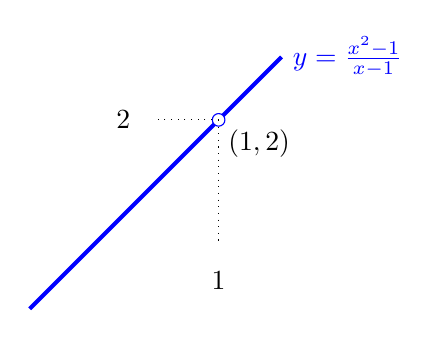
\begin{tikzpicture}[scale = 0.8]
\axes{-2}{2}{-1}{3};
\draw[blue, line width = 0.05cm] plot[domain = -2:2] (\x, {\x+1}) node[right] {$y=\frac{x^2-1}{x-1}$};
\filldraw[fill = white, draw = blue] (1, 2) circle [radius = 0.1cm] node [below right] {$(1,2)$};
\draw[dotted] (1,2) -- (1,0) node[below = 0.2cm] {$1$};
\draw[dotted] (1,2) -- (0,2) node[left = 0.2cm] {$2$};
\end{tikzpicture}
\caption{กราฟของฟังก์ชัน $f(x) = \tfrac{x^2-1}{x-1}$}
\label{fig:limit_intro}
\end{figure}

นั่นคือ เมื่อ $x=1$ แล้วค่าของ $f(x)$ ควรจะมีค่าเท่ากับ $2$ แต่เราไม่สามารถเขียนอธิบายว่า $f(1) = 2$ ได้ ฉะนั้นเราจึงต้องหาคำนิยามให้กับปรากฏการณ์นี้
\end{frame}

\begin{frame}
การอธิบาย 
\begin{remark}{}
\begin{center}
เมื่อ $x$ มีค่าเท่ากับ $1$ จะได้ค่าของฟังก์ชัน $f(x)$ เท่ากับ $2$
\end{center}
\end{remark}

สามารถเขียนเป็นสัญลักษณ์คณิตศาสตร์ได้เป็น $f(1) = 2$ 

แต่สำหรับฟังก์ชัน $f(x) = \frac{x^2-1}{x-1}$ เราต้องการจะอธิบายว่า
\begin{remark}{}
\begin{center}
เมื่อ $x$ มีค่า\red{ใกล้กับ} $1$ จะได้ค่าของฟังก์ชัน $f(x)$ \red{ใกล้กับ} $2$
\end{center}
\end{remark}

สังเกตว่าเราเปลี่ยนเป็นคำว่า ``ใกล้กับ'' เนื่องจากเราไม่สามารถหาค่าของฟังก์ชันโดยตรงได้
\end{frame}

\begin{frame}
\frametitle{สัญลักษณ์ลิมิต}
คำว่า ``ใกล้กับ'' ในทางคณิตศาสตร์คือคำว่า limit (เขียนย่อเป็น lim) โดยมีวิธีเขียนดังนี้

\[ \Scale{\red{\lim_{\color{teal}{x \rightarrow 1}}} \, \blue{f(x)} = \color{purple}{2}}\]

อ่านดังนี้

\begin{center}
\red{ลิมิต} \color{teal}เมื่อ $x$ เข้าใกล้ $1$ \blue{ของฟังก์ชัน $f(x)$} \color{purple}{มีค่าเท่ากับ $2$}
\end{center}

หรือ

\begin{center}
\red{ลิมิต} \blue{ของฟังก์ชัน $f(x)$} \color{teal}เมื่อ $x$ เข้าใกล้ $1$  \color{purple}{มีค่าเท่ากับ $2$}
\end{center}
\end{frame}


\begin{frame}
\frametitle{ลิมิตจากด้านลบและด้านบวก}
คำถามต่อไปคือ คำว่า ``เข้าใกล้'' นั่นหมายถึงการเข้าใกล้จากทางใด เนื่องจากการเข้าใกล้จุด $x=1$ เข้าได้จากทางซ้ายและทางขวา ดัง\figref{fig:limit_left_right_intro}

\begin{figure}[h!]
\centering
\begin{tikzpicture}
\draw[<->] (-2,0) -- (2,0) node[right] {$x$};
\filldraw[fill = white, draw = teal] (0, 0) circle [radius = 0.1cm] node [teal, below = 0.2 cm] {$1$};
\draw[->, red] (-2, 0.5) --+ (1.9,0);
\draw[->, blue] (2, 0.5) --+ (-1.9,0);
\end{tikzpicture}
\caption{การเข้าใกล้ค่า $x=1$ จากด้านซ้าย (สีแดง) และด้านขวา (สีน้ำเงิน)}
\label{fig:limit_left_right_intro}
\end{figure}
\end{frame}

\begin{frame}
ในทางคณิตศาสตร์เราจะอ้างอิงจากแกน $x$ ซึ่งฝั่งซ้ายเป็นค่าลบ และฝั่งขวาเป็นค่าบวก ดัง\figref{fig:limit_left_right_defn}

\begin{figure}[h!]
\centering
\begin{tikzpicture}
\draw[->] (0,0) -- (-2,0) node[left, red] {แกน $x$ ด้านลบ};
\draw[->] (0,0) -- (2,0) node[right, blue] {แกน $x$ ด้านบวก};
\filldraw[fill = white, draw = teal] (0, 0) circle [radius = 0.1cm] node [teal, below = 0.2 cm] {$1$};
\draw[->, red] (-2, 0.5) --+ (1.9,0) node[pos = 0.5, above] {ลิมิตทางซ้าย};
\draw[->, blue] (2, 0.5) --+ (-1.9,0) node[pos = 0.5, above] {ลิมิตทางขวา};
\end{tikzpicture}
\caption{ลิมิตทางซ้าย (สีแดง) และลิมิตทางขวา (สีน้ำเงิน)}
\label{fig:limit_left_right_defn}
\end{figure}
โดยจะใช้เครื่องหมาย $-$ และ $+$ เพิ่มไว้ด้านหลังค่า $x$ ดังนี้
\[\Scale{\red{\limx{1^{-}} f(x)}} \quad \text{ และ } \quad \Scale{\blue{\limx{1^{+}} f(x)}}\]
\end{frame}


\begin{frame}
\frametitle{นิยามของลิมิตทางซ้ายและทางขวา}

\begin{defn}{}{}
\textbf{ลิมิตทางซ้าย} เขียนแทนด้วย 
\[\limx{a^{-}} f(x)\]
อ่านว่า ``ลิมิตเมื่อ $x$ เข้าใกล้ $a$ จากด้านลบของฟังก์ชัน $f(x)$''  \pa

\textbf{ลิมิตทางขวา} เขียนแทนด้วย 
\[\limx{a^{+}} f(x)\]
อ่านว่า ``ลิมิตเมื่อ $x$ เข้าใกล้ $a$ จากด้านบวกของฟังก์ชัน $f(x)$'' 
\end{defn}
\end{frame}

\begin{frame}
\frametitle{นิยามของลิมิต}
เมื่อเรานิยามลิมิตทางซ้ายและขวาได้แล้ว จึงจะสามารถนิยามลิมิต ณ จุดนั้นได้
\begin{defn}{}{}
กำหนดฟังก์ชัน $f(x)$ และจำนวนจริง $a$ ที่มีเงื่อนไขดังต่อไปนี้ \pa
\begin{enumerate}
\item ลิมิตทางซ้ายและทางขวาที่จุด $x=a$ หาค่าได้ และ
\item ลิมิตทางซ้ายและทางขวามีค่าเท่ากัน
\end{enumerate}
แล้วจะนิยาม $\limx{a} f(x)$ ว่าหาค่าได้ และจะมีค่าเท่ากับลิมิตทางซ้ายและทางขวา
\end{defn}
\end{frame}

\begin{frame}
\frametitle{การลู่เข้าและลู่ออก}
นอกจากคำว่า ``หาค่าได้'' และ ``หาค่าไม่ได้'' แล้วเรามีคำที่ใช้จำแนกลิมิตอีก 2 คำ ดังนี้
\begin{defn}{}{}
ถ้า $\limx{a} f(x)$ หาค่าได้ เราจะเรียกลิมิตนี้ว่าเป็นลิมิตที่ \textbf{ลู่เข้า} (convergent)

ถ้า $\limx{a} f(x)$ หาค่าไม่ได้ เราจะเรียกลิมิตนี้ว่าเป็นลิมิตที่ \textbf{ลู่ออก} (divergent)
\end{defn}
โดยทั่วไป คำว่า ``หาค่าได้'' และ ``ลู่เข้า'' สามารถใช้แทนกันได้ แต่มีบางกรณีที่สองคำที่มีความหมายต่างกัน ซึ่งเราจะได้ศึกษาในภายหลัง
\end{frame}

%%%%%%%%%%%%%%
\section[ลิมิตจากกราฟ]{การหาลิมิตจากการวิเคราะห์กราฟ}
\frame{\sectionpage}
%%%%%%%%%%%%%%

\begin{frame}
\frametitle{การหาลิมิตทางซ้ายจากการวิเคราะห์กราฟ}

ถ้ากำหนดกราฟของฟังก์ชัน $y = f(x)$ มาให้ โดยที่ไม่ระบุเฉพาะเจาะจงว่า $f(x)$ มีรูปแบบอย่างไร เราสามารถหาลิมิตได้จากนิยาม โดยประโยคคำถาม

\begin{remark}{}
\begin{center}
จงหา $\limx{a^{-}} f(x)$
\end{center}
\end{remark}

มีความหมายว่า

\begin{remark}{}
\begin{center}
เมื่อเลื่อนค่า $x$ จากแกน $x$ ด้านลบ (ทางซ้าย) เข้ามาใกล้จุด $x=a$ แล้วค่า $f(x)$ จะมีค่าเท่าไหร่
\end{center}
\end{remark}
\end{frame}

\begin{frame}
\begin{figure}[h!]
\centering
\begin{tikzpicture}[scale = 0.8]
\axes{-2}{2}{-1}{3};
\draw (-2,3) .. controls (-0.5,0) .. (1,2);
\draw (1,3) .. controls (1.5,4) .. (2,1);
\filldraw[fill = white] (1, 2) circle [radius = 0.1cm];
\filldraw[fill = black] (1, 3) circle [radius = 0.1cm];
\draw[dotted] (1,2) -- (1,0) node[below = 0.1cm] {$a$};
\begin{scope}[xshift = 6cm]
\axes{-2}{2}{-1}{3};
\filldraw[fill = white] (1, 2) circle [radius = 0.1cm];
\filldraw[fill = black] (1, 3) circle [radius = 0.1cm];
\draw[red, -{Latex[length = 0.4cm]}] (-2,3) .. controls (-0.5,0) .. (1,2);
\draw (1,3) .. controls (1.5,4) .. (2,1);
\draw[red, ->] (-2,0) -- (1,0);
\draw[dotted] (1,2) -- (1,0) node[below = 0.1cm] {$a$};
\draw[dotted, blue] (1,2) -- (0,2) node[left = 0.1cm] {$b$};
\end{scope}
\end{tikzpicture}
\caption{การหา $\limx{a^{-}} f(x)$ (ลิมิตทางซ้ายของฟังก์ชัน $y=f(x)$) จากกราฟ}
\label{fig:limit_intro}
\end{figure}
จากภาพนี้ เราสรุปได้ว่า
\[\limx{a^{-}} f(x) = b\]
นั่นคือ
\begin{center}
เมื่อ $x$ เข้าใกล้ $a$ จากทางซ้าย (แกน $x$ ด้านลบ) แล้วค่า $y$ จะเข้าใกล้ $b$
\end{center}
\end{frame}

\begin{frame}[t]
\begin{ex}
\begin{minipage}{0.4\textwidth}
จาก\figref{fig:limit_graph_ex1} จงหา
\begin{tasks}(1)
\task $\limx{-1^{-}} f(x)$
\task $\limx{0^{-}} f(x)$
\task $\limx{1^{-}} f(x)$
\end{tasks}
\end{minipage}
\begin{minipage}{0.55\textwidth}
\centering
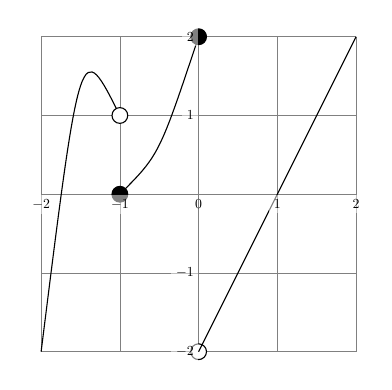
\begin{tikzpicture}
\axes{-2.2}{2.2}{-2.2}{2.2};
\draw[very thin, gray] (-2,-2) grid (2,2);
\draw (-2,-2) .. controls (-1.5,2) .. (-1,1);
\filldraw[fill = white] (-1, 1) circle [radius = 0.1cm];
\filldraw[fill = black] (-1, 0) circle [radius = 0.1cm];
\draw (-1,0) .. controls (-0.5,0.5) .. (0,2);
\filldraw[fill = black] (0, 2) circle [radius = 0.1cm];
\filldraw[fill = white] (0, -2) circle [radius = 0.1cm];
\draw (0,-2) -- (2,2);
\foreach \x in {-2,-1,1,2}
{
	\node at (\x,0) [below, scale = 0.5, fill = white, fill opacity = 0.5, text opacity = 1] {$\x$};
	\node at (0,\x) [left, scale = 0.5, fill = white, fill opacity = 0.5, text opacity = 1] {$\x$};
}
\node at (0,0) [below, scale = 0.5, fill opacity = 0.5, text opacity = 1] {$0$};
\end{tikzpicture}
\captionof{figure}{กราฟสำหรับตัวอย่างที่ \theex}
\label{fig:limit_graph_ex1}
\end{minipage}
\end{ex}
\end{frame}

\begin{frame}
\begin{figure}[h!]
\centering
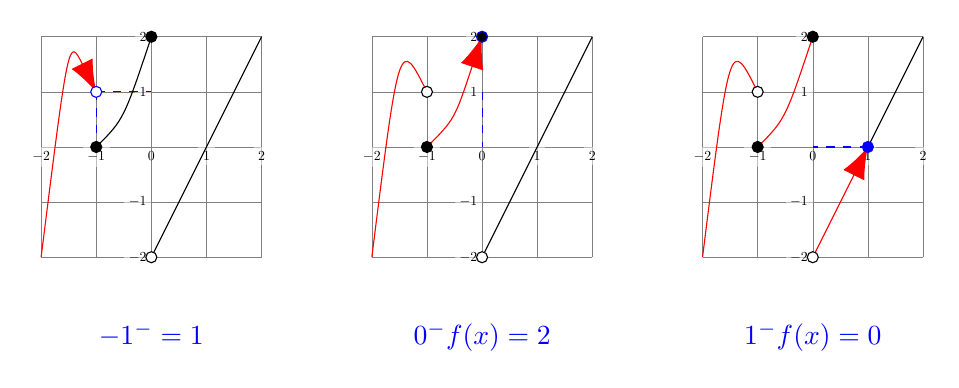
\begin{tikzpicture}[scale = 0.7]
\axes{-2.5}{2.5}{-2.5}{2.5};
\draw[very thin, gray] (-2,-2) grid (2,2);
\foreach \x in {-2,-1,1,2}
{
	\node at (\x,0) [below, scale = 0.5, fill = white, fill opacity = 0.5, text opacity = 1] {$\x$};
	\node at (0,\x) [left, scale = 0.5, fill = white, fill opacity = 0.5, text opacity = 1] {$\x$};
}

\draw[red, -{Latex[length = 0.4cm]}] (-2,-2) .. controls (-1.5,2) .. (-1,1);
\draw[blue, dashed] (-1,1) -- (-1,0);
\draw[blue, dashed] (-1,1) -- (0,1);
\filldraw[fill = white, draw = blue] (-1, 1) circle [radius = 0.1cm];
\filldraw[fill = black] (-1, 0) circle [radius = 0.1cm];
\draw (-1,0) .. controls (-0.5,0.5) .. (0,2);
\filldraw[fill = black] (0, 2) circle [radius = 0.1cm];
\draw (0,-2) -- (2,2);
\filldraw[fill = white] (0, -2) circle [radius = 0.1cm];

\node at (0,0) [below, scale = 0.5, fill opacity = 0.5, text opacity = 1] {$0$};
\node at (0,-3) [below, blue] {$\limx{-1^{-}} = 1$};
\begin{scope}[xshift = 6cm]
\axes{-2.5}{2.5}{-2.5}{2.5};
\draw[very thin, gray] (-2,-2) grid (2,2);
\foreach \x in {-2,-1,1,2}
{
	\node at (\x,0) [below, scale = 0.5, fill = white, fill opacity = 0.5, text opacity = 1] {$\x$};
	\node at (0,\x) [left, scale = 0.5, fill = white, fill opacity = 0.5, text opacity = 1] {$\x$};
}

\draw[red] (-2,-2) .. controls (-1.5,2) .. (-1,1);
\filldraw[fill = white] (-1, 1) circle [radius = 0.1cm];
\draw[red, -{Latex[length = 0.4cm]}]  (-1,0) .. controls (-0.5,0.5) .. (0,2);
\filldraw[fill = black] (-1, 0) circle [radius = 0.1cm];
\filldraw[fill = black, draw = blue] (0, 2) circle [radius = 0.1cm];
\draw (0,-2) -- (2,2);
\filldraw[fill = white] (0, -2) circle [radius = 0.1cm];

\node at (0,0) [below, scale = 0.5, fill opacity = 0.5, text opacity = 1] {$0$};
\draw[blue, dashed] (0,1) -- (0,0);
\node at (0,-3) [below, blue] {$\limx{0^{-}} f(x) = 2$};
\end{scope}
\begin{scope}[xshift = 12cm]
\axes{-2.5}{2.5}{-2.5}{2.5};
\draw[very thin, gray] (-2,-2) grid (2,2);
\foreach \x in {-2,-1,1,2}
{
	\node at (\x,0) [below, scale = 0.5, fill = white, fill opacity = 0.5, text opacity = 1] {$\x$};
	\node at (0,\x) [left, scale = 0.5, fill = white, fill opacity = 0.5, text opacity = 1] {$\x$};
}

\draw[red] (-2,-2) .. controls (-1.5,2) .. (-1,1);
\filldraw[fill = white] (-1, 1) circle [radius = 0.1cm];
\draw[red] (-1,0) .. controls (-0.5,0.5) .. (0,2);
\filldraw[fill = black] (-1, 0) circle [radius = 0.1cm];
\filldraw[fill = black] (0, 2) circle [radius = 0.1cm];
\draw[red, -{Latex[length = 0.4cm]}] (0,-2) -- (1,0);
\draw (1,0) -- (2,2);
\filldraw[blue] (1, 0) circle [radius = 0.1cm];
\filldraw[fill = white] (0, -2) circle [radius = 0.1cm];

\node at (0,0) [below, scale = 0.5, fill opacity = 0.5, text opacity = 1] {$0$};
\draw[blue, dashed] (1,0) -- (0,0);
\node at (0,-3) [below, blue] {$\limx{1^{-}} f(x) = 0$};
\end{scope}
\end{tikzpicture}
\caption{วิธีทำสำหรับตัวอย่างที่ \theex}
\label{fig:limit_graph_ex1_sol}
\end{figure}
\end{frame}


\begin{frame}
\frametitle{การหาลิมิตทางขวาจากการวิเคราะห์กราฟ}

ในทำนองเดียวกัน ประโยคคำถาม

\begin{remark}{}
\begin{center}
จงหา $\limx{a^{+}} f(x)$
\end{center}
\end{remark}

มีความหมายว่า

\begin{remark}{}
\begin{center}
เมื่อเลื่อนค่า $x$ จากแกน $x$ ด้านบวก (ทางขวา) เข้ามาใกล้จุด $x=a$ แล้วค่า $f(x)$ จะมีค่าเท่าไหร่
\end{center}
\end{remark}
\end{frame}

\begin{frame}
\begin{figure}[h!]
\centering
\begin{tikzpicture}[scale = 0.8]
\axes{-2}{2}{-1}{3};
\draw (-2,3) .. controls (-0.5,0) .. (1,2);
\draw (1,3) .. controls (1.5,4) .. (2,1);
\filldraw[fill = white] (1, 2) circle [radius = 0.1cm];
\filldraw[fill = black] (1, 3) circle [radius = 0.1cm];
\draw[dotted] (1,2) -- (1,0) node[below = 0.1cm] {$a$};
\begin{scope}[xshift = 6cm]
\axes{-2}{2}{-1}{3};
\filldraw[fill = white] (1, 2) circle [radius = 0.1cm];
\filldraw[fill = black] (1, 3) circle [radius = 0.1cm];
\draw(-2,3) .. controls (-0.5,0) .. (1,2);
\draw[red, {Latex[length = 0.4cm]}-] (1,3) .. controls (1.5,4) .. (2,1);
\draw[red, ->] (2,0) -- (1,0);
\draw[dotted] (1,3) -- (1,0) node[below = 0.1cm] {$a$};
\draw[dotted, blue] (1,3) -- (0,3) node[left = 0.1cm] {$b$};
\end{scope}
\end{tikzpicture}
\caption{การหา $\limx{a^{+}} f(x)$ (ลิมิตทางขวาของฟังก์ชัน $y=f(x)$) จากกราฟ}
\label{fig:limit_intro}
\end{figure}
จากภาพนี้ เราสรุปได้ว่า
\[\limx{a^{+}} f(x) = b\]
นั่นคือ
\begin{center}
เมื่อ $x$ เข้าใกล้ $a$ จากทางขวา (แกน $x$ ด้านบวก) แล้วค่า $y$ จะเข้าใกล้ $b$
\end{center}
\end{frame}

\begin{frame}[t]
\begin{ex}
\begin{minipage}{0.4\textwidth}
จาก\figref{fig:limit_graph_ex2} จงหา
\begin{tasks}(1)
\task $\limx{0^{+}} f(x)$
\task $\limx{-1^{+}} f(x)$
\task $\limx{-2^{+}} f(x)$
\end{tasks}
\end{minipage}
\begin{minipage}{0.55\textwidth}
\centering
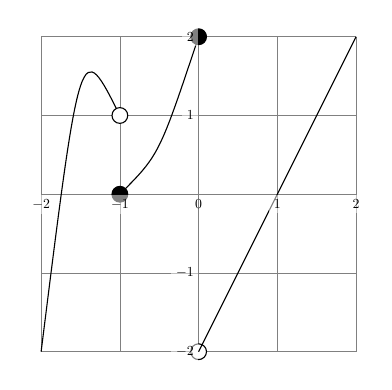
\begin{tikzpicture}
\axes{-2.2}{2.2}{-2.2}{2.2};
\draw[very thin, gray] (-2,-2) grid (2,2);
\draw (-2,-2) .. controls (-1.5,2) .. (-1,1);
\filldraw[fill = white] (-1, 1) circle [radius = 0.1cm];
\filldraw[fill = black] (-1, 0) circle [radius = 0.1cm];
\draw (-1,0) .. controls (-0.5,0.5) .. (0,2);
\filldraw[fill = black] (0, 2) circle [radius = 0.1cm];
\filldraw[fill = white] (0, -2) circle [radius = 0.1cm];
\draw (0,-2) -- (2,2);
\foreach \x in {-2,-1,1,2}
{
	\node at (\x,0) [below, scale = 0.5, fill = white, fill opacity = 0.5, text opacity = 1] {$\x$};
	\node at (0,\x) [left, scale = 0.5, fill = white, fill opacity = 0.5, text opacity = 1] {$\x$};
}
\node at (0,0) [below, scale = 0.5, fill opacity = 0.5, text opacity = 1] {$0$};
\end{tikzpicture}
\captionof{figure}{กราฟสำหรับตัวอย่างที่ \theex}
\label{fig:limit_graph_ex2}
\end{minipage}
\end{ex}
\end{frame}

\begin{frame}
\begin{figure}[h!]
\centering
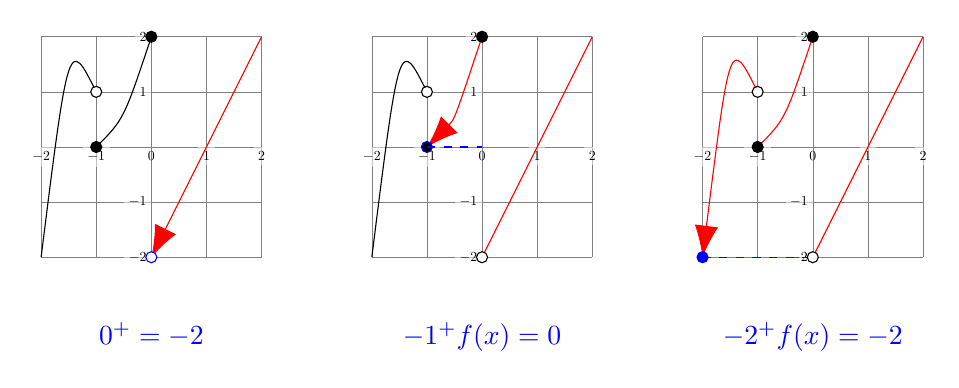
\begin{tikzpicture}[scale = 0.7]
\axes{-2.5}{2.5}{-2.5}{2.5};
\draw[very thin, gray] (-2,-2) grid (2,2);
\foreach \x in {-2,-1,1,2}
{
	\node at (\x,0) [below, scale = 0.5, fill = white, fill opacity = 0.5, text opacity = 1] {$\x$};
	\node at (0,\x) [left, scale = 0.5, fill = white, fill opacity = 0.5, text opacity = 1] {$\x$};
}

\draw(-2,-2) .. controls (-1.5,2) .. (-1,1);
\filldraw[fill = white] (-1, 1) circle [radius = 0.1cm];
\filldraw[fill = black] (-1, 0) circle [radius = 0.1cm];
\draw (-1,0) .. controls (-0.5,0.5) .. (0,2);
\filldraw[fill = black] (0, 2) circle [radius = 0.1cm];
\draw[red, {Latex[length = 0.4cm]}-] (0,-2) -- (2,2);
\filldraw[fill = white, draw = blue] (0, -2) circle [radius = 0.1cm];
\node at (0,0) [below, scale = 0.5, fill opacity = 0.5, text opacity = 1] {$0$};
\node at (0,-3) [below, blue] {$\limx{0^{+}} = -2$};
\begin{scope}[xshift = 6cm]
\axes{-2.5}{2.5}{-2.5}{2.5};
\draw[very thin, gray] (-2,-2) grid (2,2);
\foreach \x in {-2,-1,1,2}
{
	\node at (\x,0) [below, scale = 0.5, fill = white, fill opacity = 0.5, text opacity = 1] {$\x$};
	\node at (0,\x) [left, scale = 0.5, fill = white, fill opacity = 0.5, text opacity = 1] {$\x$};
}

\draw (-2,-2) .. controls (-1.5,2) .. (-1,1);
\filldraw[fill = white] (-1, 1) circle [radius = 0.1cm];
\draw[red, {Latex[length = 0.4cm]}-] (-1,0) .. controls (-0.5,0.5) .. (0,2);
\filldraw[fill = black, draw = blue] (-1, 0) circle [radius = 0.1cm];
\filldraw[fill = black] (0, 2) circle [radius = 0.1cm];
\draw[red] (0,-2) -- (2,2);
\filldraw[fill = white] (0, -2) circle [radius = 0.1cm];

\node at (0,0) [below, scale = 0.5, fill opacity = 0.5, text opacity = 1] {$0$};
\draw[blue, dashed] (-1,0) -- (0,0);
\node at (0,-3) [below, blue] {$\limx{-1^{+}} f(x) = 0$};
\end{scope}
\begin{scope}[xshift = 12cm]
\axes{-2.5}{2.5}{-2.5}{2.5};
\draw[very thin, gray] (-2,-2) grid (2,2);
\foreach \x in {-2,-1,1,2}
{
	\node at (\x,0) [below, scale = 0.5, fill = white, fill opacity = 0.5, text opacity = 1] {$\x$};
	\node at (0,\x) [left, scale = 0.5, fill = white, fill opacity = 0.5, text opacity = 1] {$\x$};
}

\draw[red, {Latex[length = 0.4cm]}-] (-2,-2) .. controls (-1.5,2) .. (-1,1);
\filldraw[fill = white] (-1, 1) circle [radius = 0.1cm];
\draw[red] (-1,0) .. controls (-0.5,0.5) .. (0,2);
\filldraw[fill = black] (-1, 0) circle [radius = 0.1cm];
\filldraw[fill = black] (0, 2) circle [radius = 0.1cm];
\draw[red] (0,-2) -- (2,2);
\filldraw[blue] (-2, -2) circle [radius = 0.1cm];
\draw[blue, dashed] (-2,-2) -- (0,-2);
\filldraw[fill = white] (0, -2) circle [radius = 0.1cm];

\node at (0,0) [below, scale = 0.5, fill opacity = 0.5, text opacity = 1] {$0$};
\node at (0,-3) [below, blue] {$\limx{-2^{+}} f(x) = -2$};
\end{scope}
\end{tikzpicture}
\caption{วิธีทำสำหรับตัวอย่างที่ \theex}
\label{fig:limit_graph_ex2_sol}
\end{figure}
\end{frame}

\begin{frame}
\frametitle{การหาลิมิตจากการวิเคราะห์กราฟ}

สุดท้าย ประโยคคำถาม

\begin{remark}{}
\begin{center}
จงหา $\limx{a} f(x)$
\end{center}
\end{remark}

มีความหมายว่า

\begin{remark}{}
\begin{center}
จงหา $\limx{a^{-}}f(x)$ และ $\limx{a^{+}}f(x)$ 

และพิจารณาว่าลิมิตทั้งสองข้างเท่ามีค่ากันหรือไม่
\end{center}
\end{remark}
\end{frame}

\begin{frame}
\begin{figure}[h!]
\centering
\begin{tikzpicture}[scale = 0.6]
\axes{-2}{2}{-1}{3};
\filldraw[fill = white] (1, 2) circle [radius = 0.1cm];
\filldraw[fill = black] (1, 3) circle [radius = 0.1cm];
\draw[blue, -{Latex[length = 0.4cm]}] (-2,3) .. controls (-0.5,0) .. (1,2);
\draw[red, {Latex[length = 0.4cm]}-] (1,3) .. controls (1.5,4) .. (2,1);
\draw[dotted] (1,3) -- (1,0) node[below = 0.1cm] {$a$};
\draw[dotted, blue] (1,2) -- (0,2) node[left = 0.1cm] {$b$};
\draw[dotted, red] (1,3) -- (0,3) node[left = 0.1cm] {$c$};
\node[scale = 0.9] at (0,-2) {$\blue{\limx{a^{-}}f(x)}$ และ $\red{\limx{a^{+}}f(x)}$ มีค่าไม่เท่ากัน};
\node[scale = 0.9] at (0,-3) {$\limx{a}f(x)$ หาค่าไม่ได้};
\begin{scope}[xshift = 10cm]
\axes{-2}{2}{-1}{3};
\filldraw[fill = white] (1, 2) circle [radius = 0.1cm];
\filldraw[fill = black] (1, 1) circle [radius = 0.1cm];
\draw[blue, -{Latex[length = 0.4cm]}] (-2,3) .. controls (-0.5,0) .. (1,2);
\draw[red, {Latex[length = 0.4cm]}-] (1,2) .. controls (1.5,3) .. (2,1);
\draw[dotted] (1,2) -- (1,0) node[below = 0.1cm] {$a$};
\draw[dotted, blue] (1,2) -- (0,2) node[left = 0.1cm] {$b$};
\node[scale = 0.9]  at (0,-2) {$\blue{\limx{a^{-}}f(x)}$ และ $\red{\limx{a^{+}}f(x)}$ เท่ากับ $b$ ทั้งคู่};
\node[scale = 0.9]  at (0,-3) {$\limx{a}f(x) = b$ };
\end{scope}
\end{tikzpicture}
\caption{การหา $\limx{a} f(x)$ จากกราฟ}
\label{fig:limit_both_intro}
\end{figure}
สังเกตในภาพฝั่งขวาว่า แม้ว่า $f(a)$ จะมีค่าไม่เท่ากับ $b$ (จากจุดสีดำ) แต่เราสรุปว่า $\limx{a}f(x) = b$ เนื่องจากการคำนวณลิมิตจะไม่สนใจค่าที่แท้จริงของ $f(a)$ แต่จะดูจากการเข้าใกล้ค่า $x=a$
\end{frame}

\begin{frame}[t]
\begin{ex}
\begin{minipage}{0.4\textwidth}
จาก\figref{fig:limit_graph_ex3} จงหา
\begin{tasks}(1)
\task $\limx{-1} f(x)$
\task $\limx{0} f(x)$
\task $\limx{1} f(x)$
\end{tasks}
\end{minipage}
\begin{minipage}{0.55\textwidth}
\centering
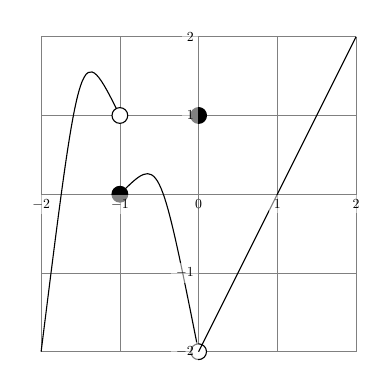
\begin{tikzpicture}
\axes{-2.2}{2.2}{-2.2}{2.2};
\draw[very thin, gray] (-2,-2) grid (2,2);
\draw (-2,-2) .. controls (-1.5,2) .. (-1,1);
\filldraw[fill = white] (-1, 1) circle [radius = 0.1cm];
\filldraw[fill = black] (-1, 0) circle [radius = 0.1cm];
\draw (-1,0) .. controls (-0.5,0.5) .. (0,-2);
\filldraw[fill = black] (0, 1) circle [radius = 0.1cm];
\filldraw[fill = white] (0, -2) circle [radius = 0.1cm];
\draw (0,-2) -- (2,2);
\foreach \x in {-2,-1,1,2}
{
	\node at (\x,0) [below, scale = 0.5, fill = white, fill opacity = 0.5, text opacity = 1] {$\x$};
	\node at (0,\x) [left, scale = 0.5, fill = white, fill opacity = 0.5, text opacity = 1] {$\x$};
}
\node at (0,0) [below, scale = 0.5, fill opacity = 0.5, text opacity = 1] {$0$};
\end{tikzpicture}
\captionof{figure}{กราฟสำหรับตัวอย่างที่ \theex}
\label{fig:limit_graph_ex3}
\end{minipage}
\end{ex}
\end{frame}

\begin{frame}
\begin{figure}[h!]
\centering
\begin{tikzpicture}[scale = 0.7]
\axes{-2.5}{2.5}{-2.5}{2.5};
\draw[very thin, gray] (-2,-2) grid (2,2);
\foreach \x in {-2,-1,1,2}
{
	\node at (\x,0) [below, scale = 0.5, fill = white, fill opacity = 0.5, text opacity = 1] {$\x$};
	\node at (0,\x) [left, scale = 0.5, fill = white, fill opacity = 0.5, text opacity = 1] {$\x$};
}
\draw[blue, -{Latex[length = 0.3cm]}] (-2,-2) .. controls (-1.5,2) .. (-1,1);
\filldraw[fill = white] (-1, 1) circle [radius = 0.1cm];
\filldraw[fill = black] (-1, 0) circle [radius = 0.1cm];
\draw[red, {Latex[length = 0.3cm]}-] (-1,0) .. controls (-0.5,0.5) .. (0,-2);
\filldraw[fill = black] (0, 1) circle [radius = 0.1cm];
\draw[red] (0,-2) -- (2,2);
\filldraw[fill = white, draw = blue] (0, -2) circle [radius = 0.1cm];
\node at (0,0) [below, scale = 0.5, fill opacity = 0.5, text opacity = 1] {$0$};
\node at (0,-3) [below, blue] {$\limx{-1^{-}} f(x) = 1$};
\node at (0,-4) [below, red] {$\limx{-1^{+}} f(x) = 0$};
\node at (0,-5) [below] {$\limx{-1} f(x)$ หาค่าไม่ได้};
\begin{scope}[xshift = 6cm]
\axes{-2.5}{2.5}{-2.5}{2.5};
\draw[very thin, gray] (-2,-2) grid (2,2);
\foreach \x in {-2,-1,1,2}
{
	\node at (\x,0) [below, scale = 0.5, fill = white, fill opacity = 0.5, text opacity = 1] {$\x$};
	\node at (0,\x) [left, scale = 0.5, fill = white, fill opacity = 0.5, text opacity = 1] {$\x$};
}

\draw[blue] (-2,-2) .. controls (-1.5,2) .. (-1,1);
\filldraw[fill = white] (-1, 1) circle [radius = 0.1cm];
\draw[blue, -{Latex[length = 0.3cm]}] (-1,0) .. controls (-0.5,0.5) .. (0,-2);
\filldraw[fill = black, draw = blue] (-1, 0) circle [radius = 0.1cm];
\filldraw[fill = black] (0, 1) circle [radius = 0.1cm];
\draw[red, {Latex[length = 0.3cm]}-] (0,-2) -- (2,2);
\filldraw[fill = white] (0, -2) circle [radius = 0.1cm];

\node at (0,0) [below, scale = 0.5, fill opacity = 0.5, text opacity = 1] {$0$};
\node at (0,-3) [below, blue] {$\limx{-1^{-}} f(x) = -2$};
\node at (0,-4) [below, red] {$\limx{-1^{+}} f(x) = -2$};
\node at (0,-5) [below] {$\limx{-1} f(x) = -2$};
\end{scope}
\begin{scope}[xshift = 12cm]
\axes{-2.5}{2.5}{-2.5}{2.5};
\draw[very thin, gray] (-2,-2) grid (2,2);
\foreach \x in {-2,-1,1,2}
{
	\node at (\x,0) [below, scale = 0.5, fill = white, fill opacity = 0.5, text opacity = 1] {$\x$};
	\node at (0,\x) [left, scale = 0.5, fill = white, fill opacity = 0.5, text opacity = 1] {$\x$};
}

\draw[blue] (-2,-2) .. controls (-1.5,2) .. (-1,1);
\filldraw[fill = white] (-1, 1) circle [radius = 0.1cm];
\draw[blue] (-1,0) .. controls (-0.5,0.5) .. (0,-2);
\filldraw[fill = black] (-1, 0) circle [radius = 0.1cm];
\filldraw[fill = black] (0, 1) circle [radius = 0.1cm];
\draw[blue, -{Latex[length = 0.4cm]}] (0,-2) -- (1,0);
\draw[red, {Latex[length = 0.4cm]}-] (1,0) -- (2,2);
\filldraw[fill = white] (0, -2) circle [radius = 0.1cm];

\node at (0,0) [below, scale = 0.5, fill opacity = 0.5, text opacity = 1] {$0$};
\node at (0,-3) [below, blue] {$\limx{1^{-}} f(x) = 0$};
\node at (0,-4) [below, red] {$\limx{1^{+}} f(x) = 0$};
\node at (0,-5) [below] {$\limx{1} f(x) = 0$};
\end{scope}
\end{tikzpicture}
\caption{วิธีทำสำหรับตัวอย่างที่ \theex}
\label{fig:limit_graph_ex3_sol}
\end{figure}
\end{frame}

%%%%%%%%%%%%%%
\section[ลิมิตจากฟังก์ชัน]{การหาลิมิตจากการวิเคราะห์ฟังก์ชัน}
\frame{\sectionpage}
%%%%%%%%%%%%%%

\begin{frame}[t]
\frametitle{การหาลิมิตทางซ้ายหรือทางขวาจากการวิเคราะห์ฟังก์ชัน}
แม้ว่าการหาลิมิตจากกราฟจะใช้การสังเกตได้ง่าย แต่ในทางปฏิบัติเราต้องใช้การคำนวณและพิสูจน์เชิงประจักษ์ พิจารณาโจทย์ปัญหาต่อไปนี้
\begin{remark}{}
\begin{center}
จงหา $\limx{1^{-}} f(x)$ เมื่อกำหนดให้ $f(x) = \frac{x^2-1}{x-1}$
\end{center}
\end{remark}

\begin{slide}
จากนิยาม โจทย์นี้มีความหมายดังนี้
\begin{remark}{}
\begin{center}
เมื่อเลื่อนค่า $x$ จากแกน $x$ ด้านลบ เข้ามาใกล้จุด $x=1$ แล้วค่า $f(x)$ จะมีค่าเท่าไหร่
\end{center}
\end{remark}
\end{slide}
\end{frame}

\begin{frame}[t]
ซึ่งเราแสดงการเลื่อนเข้ามาใกล้จากด้านลบ ด้วยลำดับของตัวเลขที่น้อยกว่า $1$ และมีค่าเข้าใกล้ $1$ ได้ เช่น
\begin{slide}
เราอาจจะหยิบยกลำดับเป็น
\[-3, -2,-1,0\]
หรือถ้าต้องการความละเอียด เราอาจจะหยิบลำดับ
\[0.9, 0.99, 0.99, 0.999\]
โดยที่ไม่มีกฎตายตัวในการเลือกลำดับ แต่ที่นิยมใช้บ่อยในการหาลิมิตทางซ้าย $\limx{a^{-}} f(x)$ คือ
\[a - 0.1, a - 0.01, a - 0.001, \ldots\]
ส่วนถ้าจะหาลิมิตทางขวา $\limx{a^{+}}f(x)$ จะนิยมหยิบลำดับ
\[a + 0.1, a + 0.01, a + 0.001, \ldots\]
ขึ้นอยู่กับว่าเราต้องการความละเอียดเท่าไหร่
\end{slide}
\end{frame}

\begin{frame}
\begin{figure}[h!]
\centering
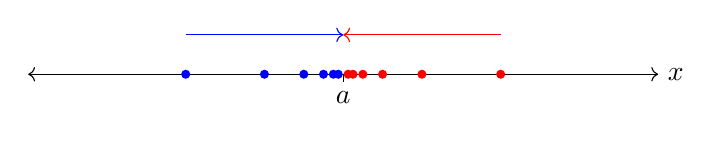
\begin{tikzpicture}
\draw[<->] (-4,0) -- (4,0) node[right] {$x$};
\draw (0,0) -- (0, -0.1) node[below] {$a$};
\draw[->, blue] (-2, 0.5) -- (0,0.5);
\draw[->, red] (2, 0.5) -- (0,0.5);
\foreach \x in {-1,0, 1,2,3,4}
{
	\filldraw[blue] ({-(2^(-\x))}, 0) circle [radius = 0.05cm];
	\filldraw[red] ({2^(-\x))}, 0) circle [radius = 0.05cm];
}
\end{tikzpicture}
\caption{ตัวอย่างการเลือกลำดับที่เข้าใกล้ $a$ จากด้านลบ (สีน้ำเงิน) และเข้าใกล้ $a$ จากด้านบวก (สีแดง)}
\label{fig:limit_numerical_seq}
\end{figure}
\end{frame}


\begin{frame}[t]
\begin{ex}
กำหนดให้ $f(x) = \frac{x^2-1}{x-1}$ จงสร้างตารางค่าของ $f(x)$ เมื่อให้ $x = 0.9, 0.99, 0.999$ และคาดเดาค่าของ $\limx{1^{-}}f(x)$ 
\end{ex}
\begin{sol}
สร้างตารางตามคำสั่งได้ดังนี้
\begin{table}[h!]
\centering
\begin{tblr}{cells={$}, colspec={|c||X[c]|X[c]|X[c]|}, rowspec={|Q|Q|}}
x & 0.9 & 0.99 & 0.999 \\
f(x) = \tfrac{x^2-1}{x-1} \pa & \tfrac{0.9^2-1}{0.9-1} = 1.9 \pa & \tfrac{0.99^2-1}{0.99-1} = 1.99 & \tfrac{0.999^2-1}{0.999-1} = 1.999\\
\end{tblr}
\end{table}
จากตาราง เมื่อค่า $x$ เข้าใกล้ $1$ จากด้านลบ แล้วค่าของ $f(x)$ เป็น $1.9, 1.99$ และ $1.999$ ซึ่งมีแนวโน้มเข้าใกล้ $2$ ดังนั้นเราจึงคาดเดาว่า $\limx{1^{-}}f(x) = 2$
\end{sol}
\end{frame}


\begin{frame}[t]
\begin{ex}
กำหนดให้ $f(x) = \frac{x^2-1}{x-1}$ จงสร้างตารางค่าของ $f(x)$ เมื่อให้ $x = 1.1, 1.01, 1.001$ และคาดเดาค่าของ $\limx{1^{+}}f(x)$ 
\end{ex}
\begin{sol}
สร้างตารางตามคำสั่งได้ดังนี้
\begin{table}[h!]
\centering
\begin{tblr}{cells={$}, colspec={|c||X[c]|X[c]|X[c]|}, rowspec={|Q|Q|}}
x & 1.1 & 1.01 & 1.001 \pa \\
f(x) = \tfrac{x^2-1}{x-1} \pa & \frac{1.1^2-1}{1.1-1} = 2.1 \pa & \frac{1.01^2-1}{1.01-1} = 2.01 \pa & \frac{1.001^2-1}{1.001-1} = 2.001\\
\end{tblr}
\end{table}\pa
จากตาราง เมื่อค่า $x$ เข้าใกล้ $1$ จากด้านบวก แล้วค่าของ $f(x)$ เป็น $2.1, 2.01$ และ $2.001$ ซึ่งมีแนวโน้มเข้าใกล้ $2$ ดังนั้นเราจึงคาดเดาว่า $\limx{1^{+}}f(x) = 2$
\end{sol}
\end{frame}


\begin{frame}
\frametitle{การหาลิมิตจากการวิเคราะห์ฟังก์ชัน}
ในทำนองเดียวกัน สำหรับโจทย์ปัญหาลิมิต
\begin{remark}{}
\begin{center}
จงหา $\limx{1} f(x)$ เมื่อกำหนดให้ $f(x) = \frac{x^2-1}{x-1}$
\end{center}
\end{remark}

สามารถทำได้ด้วยการวิเคราะห์ลิมิตทางซ้ายและทางขวาแยกกัน ซึ่งถ้าเราใช้ตารางแล้วเราจะสามารถทำพร้อมกันเลยได้
\end{frame}

\begin{frame}[t]
\begin{ex}
กำหนดให้ $f(x) = \frac{|x|}{x} $ จงสร้างตารางค่าของ $f(x)$ เมื่อให้ $x = -0.1, -0.01, -0.001, 0.001, 0.01, 0.1$ และคาดเดาค่าของ $\limx{0}f(x)$ 
\end{ex}
\begin{sol}
สร้างตารางตามคำสั่งได้ดังนี้
\begin{table}[h!]
\centering
\begin{tblr}{cells={$}, colspec={|c||X[c]|X[c]|X[c]|X[c]|X[c]|X[c]|}, rowspec={|Q|Q|}}
x & -0.1 & -0.01 & -0.001 & 0.001 & 0.01 & 0.1 \\
\pa \displaystyle f(x) = \frac{x}{|x|} & \pa -1&  \pa -1 & \pa-1 & \pa 1 & \pa 1 & \pa 1\\
\end{tblr}
\end{table} 
สังเกตว่า $\limx{0^{-}} f(x)$ มีแนวโน้มเข้าใกล้ค่า $-1$ แต่ $\limx{0^{+}} f(x)$ มีแนวโน้มเข้าใกล้ค่า $1$ เนื่องจากลิมิตซ้ายและลิมิตขวามีค่าไม่เท่ากัน เราจึงคาดเดาว่า $\limx{0} f(x)$ หาค่าไม่ได้
\end{sol}
\end{frame}



%%%%%%%%%%%%%%
\section{การคำนวณลิมิต}
\frame{\sectionpage}
%%%%%%%%%%%%%%

\begin{frame}[t]
\frametitle{ความสำคัญของการคำนวณลิมิต}
ถึงแม้เราจะใช้กราฟหรือสร้างตารางค่าของฟังก์ชันมาช่วยวิเคราะห์ แต่เราก็ยังไม่ได้พิสูจน์อย่างชัดเจนว่าลิมิตหาค่าได้จริงหรือไม่ เราจึงต้องหาวิธีการคำนวณที่ได้ผลลัพธ์แน่นอน เช่น

\medskip

สำหรับฟังก์ชันพื้นฐานที่ใช้งานบ่อยและคำนวณได้ง่าย เราสามารถสร้างทฤษฎีบทต่อยอดกันได้ 

พิจารณา 
\[\limx{a} f(x)\]
เมื่อ $f(x)$ เป็นค่าคงตัว และเมื่อ $f(x) = x$
\end{frame}

\begin{frame}[t]
\begin{figure}[h!]
\centering
\begin{tikzpicture}
\axes{-2}{2}{-1}{2};
\draw[blue, line width = 0.03cm] (-2,1) -- (2,1) node[right] {$f(x) = c$};
\draw (0.1,1) -- (-0.1,1) node[below left] {$c$};
\draw[red, ->] (-2, 1.5) -- (0.8,1.5);
\draw[red, ->] (2, 1.5) -- (1.2,1.5);
\draw[dashed] (1,1) -- (1,-0.1) node[below] {$a$};
\filldraw[blue] (1,1) circle [radius = 0.05cm];
\end{tikzpicture}
\captionof{figure}{กราฟแสดง $\limx{a} f(x)$ เมื่อ $f(x) = c$}
\label{fig:limit_prop_constant}
\end{figure}
จากกราฟ จะเห็นว่าลิมิตทางซ้ายและทางขวาต่างก็มีค่าเท่ากับ $c$ ฉะนั้น
\begin{remark}{}
\[ \limx{a} c = c \]
\end{remark}
\end{frame}

\begin{frame}[t]
\begin{figure}[h!]
\centering
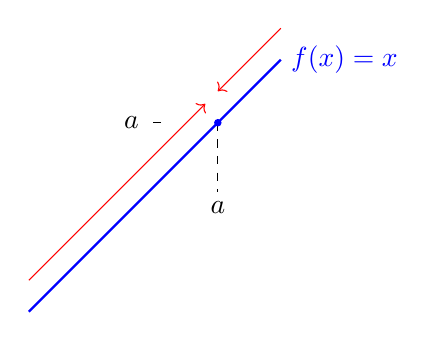
\begin{tikzpicture}[scale = 0.8]
\axes{-2}{2}{-2}{2};
\draw[blue, line width = 0.03cm] (-2,-2) -- (2,2) node[right] {$f(x) = x$};
\draw[red, ->] (-2, -1.5) -- (0.8,1.3);
\draw[red, ->] (2, 2.5) -- (1,1.5);
\draw[dashed] (1,1) -- (1,-0.1) node[below] {$a$};
\draw[dashed] (0.1,1) -- (-0.1,1) node[left] {$a$};
\filldraw[blue] (1,1) circle [radius = 0.05cm];
\end{tikzpicture}
\captionof{figure}{กราฟแสดง $\limx{a} f(x)$ เมื่อ $f(x) = x$}
\label{fig:limit_prop_linear}
\end{figure}
จากกราฟ จะเห็นว่าลิมิตทางซ้ายและทางขวาต่างก็เข้าใกล้ $a$ ฉะนั้น
\begin{remark}{}
\[ \limx{a} x = a \]
\end{remark}
\end{frame}


\begin{frame}
\frametitle{ทฤษฎีบทสำหรับลิมิตของฟังก์ชันพื้นฐาน}
\begin{thm}{สมบัติของลิมิต}{}
ให้ $a$ และ $c$ เป็นจำนวนจริง จะได้ว่า \pa
\begin{enumerate}
%\item \textbf{ลิมิตมีได้เพียงค่าเดียวเท่านั้น}: \pa ถ้า $\limx{a} f(x)= l$ และ $\limx{a} f(x)= m$ แล้วจะได้ว่า $ l= m$ \pa
\item $\limx{a} c = c$  \pa
\item $\limx{a} x = a$ 
\end{enumerate}
\end{thm}
\end{frame}



\begin{frame}[t]
\begin{ex}
จงหาค่าของลิมิตต่อไปนี้
\begin{tasks}(4)
\task $\limx{2} 5 $
\task $\limx{0} -4 $
\task $\limx{2} x $
\task $\limx{\pi} x$ 
\end{tasks}
\end{ex}
\begin{sol}
\begin{tasks}(1)
\task เนื่องจากฟังก์ชัน $f(x) = 5$ เป็นฟังก์ชันค่าคงตัว \pa ฉะนั้น $\limx{2} 5 = 5$ \pa
\task เนื่องจากฟังก์ชัน $f(x) = -4$ เป็นฟังก์ชันค่าคงตัว \pa ฉะนั้น $\limx{0} -4 =  -4$ \pa
\task เนื่องจากกำหนดฟังก์ชัน $f(x) = x$ มาให้ ฉะนั้น $\limx{2} x = 2$ \pa
\task เนื่องจากกำหนดฟังก์ชน $f(x) = x$ มาให้ ฉะนั้น $\limx{\pi} x = \pi$ 
\end{tasks}
\end{sol}
\end{frame}

\begin{frame}
\frametitle{ลิมิตของผลบวกและผลลบฟังก์ชัน และการคูณด้วยค่าคงตัว}
ในการหาลิมิตของฟังก์ชันพีชคณิต หรือฟังก์ชันประกอบ เราสามารถหาลิมิตของฟังก์ชันทีละฟังก์ชัน แล้วค่อยนำมาคำนวณทีหลังได้
\begin{prop}{พีชคณิตของลิมิต}{}
ถ้า $\limx{a} f(x) = L$ และ $\limx{a} g(x) = M$ จะได้ว่า \pa
\begin{enumerate}
\item $\limx{a}[f(x) \blue{+} g(x)] = \limx{a} f(x) \blue{+} \limx{a} g(x) = L\blue{+}M$ \pa
\item $\limx{a} [f(x) \blue{-} g(x)] = \limx{a} f(x) \blue{-} \limx{a} g(x) = L \blue{-} M$ \pa
\item $\limx{a} \blue{c} (f(x)) = \blue{c} \limx{a} f(x) = \blue{c} L$ เมื่อ $c$ เป็นค่าคงตัว  \pa
\end{enumerate}
\end{prop}
\end{frame}


\begin{frame}[t]
\begin{ex}
จงหาค่าของ 
\begin{tasks}(2)
\task $\limx{3} (x+ 5)$
\task $\limx{2} (3x-1 )$
\end{tasks}
\end{ex}
\begin{sol}
\begin{eqnarray*}
\limx{3} (x+ 5) \pa &=& \limx{3} x + \limx{3} 5 \pa \\
&=& 3+5 \\
&=& 8 \\
\limx{2} (3x-1 ) \pa &=& \limx{2} 3x - \limx{2} 1 \pa \\
&=& 3\limx{2} x - \limx{2} 1 \pa \\
&=& 3(2) - 1 = 5
\end{eqnarray*}
\end{sol}
\end{frame}

\begin{frame}
\frametitle{ลิมิตของผลคูณและผลหารฟังก์ชัน}
เราสามารถหาลิมิตของฟังก์ชันที่อยู่ในรูปผลคูณ หรือผลหารของฟังก์ชันได้เช่นกัน ที่ต้องระวังคือ ถ้าเป็นเป็นรูปผลหารแล้ว ตัวส่วนต้องไม่เท่ากับ 0 ถ้าตัวส่วนเท่ากับ 0 ต้องใช้วิธีอื่น ซึ่งดูได้ในหน้าถัดไป
\begin{prop}{พีชคณิตของลิมิต}{}
ถ้า $\limx{a} f(x) = L$ และ $\limx{a} g(x) = M$ จะได้ว่า \pa
\begin{enumerate}
\item $\limx{a} f(x) g(x) = \left(\limx{a} f(x)\right)\left( \limx{a} g(x)\right) = LM$ \pa
\item $\limx{a} \frac{f(x)}{g(x)} = \frac{ \limx{a} f(x)}{ \limx{a} g(x)} = \frac{L}{M}$ เมื่อ $m \neq 0$ \pa
\end{enumerate}
\end{prop}
\end{frame}


\begin{frame}[t]
\begin{ex}
จงหาค่าของ  $\limx{1} 2x(x+3)$
\end{ex}
\begin{sol}
\begin{eqnarray*}
\limx{1} 2x(x+3) \pa = 2 \limx{1} x(x+3) \pa &=& 2 (\limx{1} x)(\limx{1} x+3) \pa \\
&=& 2(\limx{1} x)(\limx{1} x + \limx{1} 3) \pa \\
&=& 2(1)(1+3) \pa\\
&=& 8 \pa \\
\end{eqnarray*}
\end{sol}
\end{frame}

\begin{frame}[t]
\begin{ex}
จงหาค่าของ $\limx{-1} \left(\frac{x-3}{x-1}\right) $
\end{ex}
\begin{sol}
\begin{eqnarray*}
\limx{-1} \left(\frac{x-3}{x-1}\right) \pa = \frac{\limx{-1} (x-3)}{\limx{-1} (x-1)} \pa &=& \frac{\left(\limx{-1} x\right) - \left(\limx{-1}3\right)}{\left(\limx{-1} x\right) - \left(\limx{-1} 1\right)} \pa \\
&=& \frac{-1-3}{-1-1} \pa = \frac{-4}{-2} \pa = 2
\end{eqnarray*}
\end{sol}
\end{frame}

\begin{frame}
\frametitle{ลิมิตของฟังก์ชันอื่น ๆ}
\begin{prop}{พีชคณิตของลิมิต (ต่อ)}{}
ถ้า $\limx{a} f(x) = L$ และ $\limx{a} g(x) = M$ จะได้ว่า \pa
\begin{enumerate}
\setcounter{enumi}{5}
\item $\limx{a} [f(x)]^{g(x)} = \left[\limx{a} f(x)\right]^{\left[\limx{a} g(x)\right]}  =L^M$ เมื่อ $L > 0$
\item ถ้า $n$ เป็นจำนวนคี่แล้ว $\limx{a} \sqrt[n]{f(x)} = \sqrt[n]{\limx{a} f(x)} = \sqrt[n]{L}$
\item ถ้า $n$ เป็นจำนวนคู่และ $L>0$ แล้ว $\limx{a} \sqrt[n]{f(x)} = \sqrt[n]{\limx{a} f(x)} = \sqrt[n]{L}$
\end{enumerate}
\end{prop}
\end{frame}


\begin{frame}[t]
\begin{ex}
จงหาค่าของ 
\begin{tasks}(3)
\task $\limx{-3} x^2 $
\task $\limx{5} \sqrt{x+4}$
\task $\limx{2} (x+2)^{x+1}$
\end{tasks}
\end{ex}
\begin{sol}
\begin{eqnarray*}
\limx{-3} x^2 \pa &=& \left(\limx{-3} x\right)^2 = (-3)^2 = 9 \pa \\
\limx{5} \sqrt{x+4} \pa &=& \sqrt{\limx{5} (x+4)} \pa = \sqrt{5+4} = \sqrt{9} = 3 \pa \\
\limx{2} (x+2)^{x+1} \pa &=& (\limx{2} (x+2))^{(\limx{2} (x+1))} \\
\pa &=& (2+2)^{(2+1)} \pa = 4^3 \pa = 64
\end{eqnarray*}
\end{sol}
\end{frame}

\begin{frame}
\frametitle{ข้อสรุป}
หลังจากที่เราเห็นตัวอย่างแล้ว สังเกตว่าเราสามารถตั้งสมมติฐานได้ดังนี้
\begin{remark}{}
\begin{center}
ถ้า $f(a)$ หาค่าได้ แล้ว $\limx{a} f(x) = f(a)$
\end{center}
\end{remark}
ซึ่งเป็นจริงสำหรับฟังก์ชันพื้นฐาน แต่ภายใต้เงื่อนไขบางอย่างฟังก์ชันของ $f(x)$ อาจทำให้ลิมิตหาค่าไม่ได้ก็ได้ เราจึงไม่สามารถสรุปเป็นทฤษฎีแบบแน่นอนได้
\end{frame}

%%%%%%%%%%%%%%
\section{ลิมิตอนันต์}
\frame{\sectionpage}
%%%%%%%%%%%%%%

\begin{frame}[t]
\begin{ex}
จงพิจารณา $\limx{0^+} f(x)$ เมื่อ $f(x) = \frac{1}{x}$ โดยใช้กราฟและตาราง
\end{ex}\pa
\begin{sol}
เมื่อวาดกราฟ สังเกตว่าเมื่อค่า $x$ เข้าใกล้ $0$ จากทางขวา เส้นโค้งจะชันขึ้นไปเรื่อย ๆ ทำให้ไม่สามารถบอกจากกราฟได้ว่าลิมิตจะเข้าค่า $y$ หรือไม่
\begin{figure}[h!]
\centering
\begin{tikzpicture}[scale = 0.7]
\axes{-1}{2}{-2}{2};
\draw[blue, line width = 0.03cm, domain = -1:-0.5] plot (\x, {1/\x});
\draw[blue, line width = 0.03cm, domain = 0.5:2, {Latex[width = 0.3cm]}-] plot (\x, {1/\x}) node [right] {$f(x) = \frac{1}{x}$};
\node at (0, -0.1) {$0$};
\end{tikzpicture}
\caption{กราฟแสดง $\limx{0^{+}} \frac{1}{x}$}
\label{fig:limit_inf_intro_undefined}
\end{figure}
\end{sol}
\end{frame}

\begin{frame}[t]
\begin{sol}
(ต่อ) เมื่อสร้างตาราง จะได้ค่าดังตารางต่อไปนี้
\begin{table}[h!]
\centering
\begin{tblr}{cells={$}, colspec={|c||X[c]|X[c]|X[c]|X[c]|}, rowspec={|Q|Q|}}
x & 0.1 & 0.01 & 0.001 & 0.0001 \\
\displaystyle f(x) = \frac{1}{x} & 10 & 100 & 1000 & 10000 \\
\end{tblr}
\end{table} 
สังเกตว่า ค่า $f(x)$ ก็จะมากขึ้นไปเรื่อย ๆ แบบไม่มีขอบเขตเช่นกัน ทำให้เราไม่สามารถหาลิมิตได้

ในที่นี้ เราจะสรุปว่า
\[ \limx{0^+} f(x) = + \infty \]
หรือ
\[ \limx{0^+} f(x) \text{ หาค่าไม่ได้}\]
ได้ทั้งคู่
\end{sol}
\end{frame}


\begin{frame}[t]
\begin{ex}
จงพิจารณา $\limx{0^-} f(x)$ เมื่อ $f(x) = \frac{1}{x}$ โดยใช้ตาราง \pa
\end{ex}
\begin{sol}
 สร้างตารางเพื่อดูค่า $f(x)$ โดยเลือกค่า $x$ บางค่าที่น้อยกว่า 0 และเข้าใกล้ 0 ดังนี้
\begin{table}[h!]
\centering
\begin{tblr}{cells={$}, colspec={|c||X[c]|X[c]|X[c]|X[c]|}, rowspec={|Q|Q|}}
x & -1 & -0.1 & -0.01 & -0.001 \pa\\
f(x) = \frac{1}{x} \pa & -1 \pa & -10 \pa & -100\pa & -1,000\\
\end{tblr}
\end{table}\pa

จะเห็นว่า ขณะเมื่อ $x$ มีเพิ่มขึ้นเรื่อย ๆ จนเข้าใกล้ 0 แล้ว $f(x)$ ก็มีค่าลดลงเรื่อย ๆ แบบไม่มีขอบเขต
\end{sol}
\end{frame}


\begin{frame}
\frametitle{นิยามฟังก์ชันที่มีลิมิตเป็นอนันต์}
การที่ค่าของฟังก์ชันมากขึ้นหรือลดลงแบบไม่มีขอบเขต เป็นกรณีพิเศษที่เรานิยามได้ดังนี้
\begin{defn}{}{}
ฟังก์ชัน $f(x)$ มีลิมิตเป็นอนันต์ที่ $x=a$ ถ้า 
\[\limx{a} f(x) = +\infty  \quad \text{หรือ} \quad \limx{a} f(x) = -\infty\]
ฟังก์ชันที่มีลิมิตเป็นอนันต์ นับเป็นฟังก์ชันที่หาลิมิตไม่ได้และลู่ออกที่จุดนั้น
\end{defn}
ฟังก์ชันเบื้องต้นที่มีลิมิตเป็นอนันต์ คือฟังก์ชันที่มีการหารด้วย $0$ เกิดขึ้น แต่มีฟังก์ชันอื่น ๆ ที่มีลิมิตเป็นอนันต์ เช่น $f(x) = \tan(x)$ ที่เราต้องศึกษาแยกเป็นฟังก์ชันไป
\end{frame}


\begin{frame}[t]
\begin{ex}
จงพิจารณา $\limx{0^+} f(x)$ เมื่อ $f(x) = \frac{1}{x^2}$ โดยใช้ตารางสำหรับค่า $x = 0.1, 0.01, 0.001$ และ $0.0001$ \pa
\end{ex}
\begin{sol}
สร้างตารางตามคำสั่งได้ดังนี้
\begin{table}[h!]
\centering
\begin{tblr}{cells={$}, colspec={|c||X[c]|X[c]|X[c]|X[c]|}, rowspec={|Q|Q|}}
x & 0.1 & 0.01 & 0.001 & 0.0001 \\
f(x) = \frac{1}{x^2} & 100 & 10000 & 100000 & 100000000\\
\end{tblr}
\end{table}\pa

จะเห็นว่า ขณะเมื่อ $x$ มีค่าลดเพิ่มขึ้นเรื่อย ๆ จนเข้าใกล้ 0 แล้ว $f(x)$ ก็มีค่าเพิ่มขึ้นเรื่อย ๆ แบบไม่มีขอบเขต เราจึงคาดเดาได้ว่า $\limx{0^+} f(x) = +\infty$
\end{sol}
\end{frame}

\begin{frame}[t]
\begin{ex}
จงพิจารณา $\limx{1^-} f(x)$ เมื่อ $f(x) = \frac{1}{x^2-x}$ โดยใช้ตารางสำหรับค่า $x = 0.9, 0.99, 0.999$ และ $0.9999$ \pa
\end{ex}
\begin{sol}
สร้างตารางตามคำสั่งได้ดังนี้
\begin{table}[h!]
\centering
\begin{tblr}{cells={$}, colspec={|c||X[c]|X[c]|X[c]|X[c]|}, rowspec={|Q|Q|}}
x & 0.1 & 0.01 & 0.001 & 0.0001 \\
f(x) = \frac{1}{x^2-x} & -11.11 & -101.01 & -1001.00 & -10001.00\\
\end{tblr}
\end{table}\pa

จะเห็นว่า ขณะเมื่อ $x$ มีค่าเพิ่มขึ้นเรื่อย ๆ จนเข้าใกล้ 1 แล้ว $f(x)$ ก็มีค่าลดลงเรื่อย ๆ แบบไม่มีขอบเขต เราจึงคาดเดาได้ว่า $\limx{1^-} f(x) = -\infty$
\end{sol}
\end{frame}


\begin{frame}
\frametitle{นิยามฟังก์ชันที่มีลิมิต ณ อนันต์}
จากตัวอย่างก่อนหน้านี้ ค่า $y$ มีค่ามากขึ้นเรื่อย ๆ ซึ่งเรานับว่าเป็นค่าอนันต์ ในทำนองเดียวกันเราก็สามารถให้ค่า $x$ มีค่ามากขึ้นเรื่อย ๆ เป็นค่าอนันต์ได้เช่นกัน
\begin{defn}{}{}
ลิมิต ณ อนันต์ของฟังก์ชัน $f(x)$ คือ
\[ \limx{+\infty} f(x) \quad \text { หรือ } \quad \limx{-\infty} f(x)\]
\end{defn}

\begin{figure}[h!]
\centering
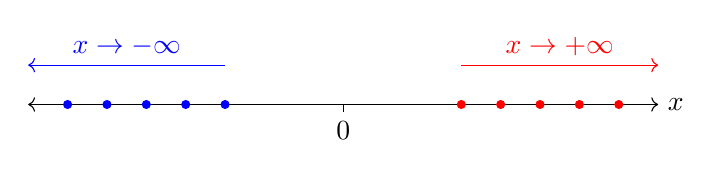
\begin{tikzpicture}
\draw[<->] (-4,0) -- (4,0) node[right] {$x$};
\draw (0,0) -- (0, -0.1) node[below] {$0$};
\draw[->, blue] (-1.5, 0.5) -- (-4,0.5) node[pos = 0.5, above] {$x \rightarrow -\infty$};
\draw[->, red] (1.5, 0.5) -- (4,0.5) node[pos = 0.5, above] {$x \rightarrow +\infty$};
\foreach \x in {0,1,2,3,4}
{
	\filldraw[blue] ({-1.5-(\x/2)}, 0) circle [radius = 0.05cm];
	\filldraw[red] ({1.5+(\x/2)}, 0) circle [radius = 0.05cm];
}
\end{tikzpicture}
\caption{ตัวอย่างลำดับที่เข้าใกล้ $-\infty$ (สีน้ำเงิน) และเข้าใกล้ $+\infty$ (สีแดง)}
\end{figure}
\end{frame}



\begin{frame}[t]
\begin{ex}
จงพิจารณา $\limx{+\infty} \frac{1}{x}$ โดยใช้ตารางและกราฟ
\end{ex}
\begin{sol}
สร้างตารางเพื่อดูค่า $f(x)$ โดยเลือกค่า $x$ ที่มีค่ามากขึ้นเรื่อย ๆ ดังนี้
\begin{table}[h!]
\centering
\begin{tblr}{cells={$}, colspec={|c||X[c]|X[c]|X[c]|X[c]|}, rowspec={|Q|Q|}}
x & 10 & 100 & 1000 & 10000 \pa\\
f(x) = \frac{1}{x} \pa & 0.1 \pa & 0.01 \pa & 0.001\pa & 0.0001\\
\end{tblr}
\end{table}\pa

จะเห็นว่า ขณะเมื่อ $x$ มีค่าเพิ่มขึ้นเรื่อย ๆ แล้ว $f(x)$ ก็มีค่าลดลงเรื่อย ๆ จนเข้าใกล้ศูนย์ เราจึงคาดเดาว่า $\limx{+\infty} f(x) = 0$

ในที่นี้ เราจะสรุปว่า
\[ \limx{0^-} f(x) = - \infty \]
หรือ
\[ \limx{0^-} f(x) \text{ หาค่าไม่ได้}\]
ได้ทั้งคู่
\end{sol}
\end{frame}

\begin{frame}[t]
\begin{sol} 
ในทำนองเดียวกัน เราสามารถพิจารณาจากกราฟได้ดังนี้
\begin{figure}[h!]
\centering
\begin{tikzpicture}
\draw[->] (0,0) -- (0,2) node [above] {$y$};
\draw[->] (0,0) -- (4,0) node [right] {$x$};
\draw[blue, line width = 0.03cm, domain = 0.5:4, -{Latex[width = 0.3cm]}] plot (\x, {1/\x}) node [above right] {$f(x) = \frac{1}{x}$};
\end{tikzpicture}
\caption{กราฟแสดง $\limx{+\infty} \frac{1}{x}$}
\label{fig:limit_inf_intro_infty}
\end{figure}

สังเกตว่า เมื่อค่า $x$ มากขึ้นเรื่อย ๆ ค่า $y$ ก็ลดลงเรื่อย ๆ เช่นกัน และเนื่องจากเราทราบว่ากราฟ $f(x) = \frac{1}{x}$ เป็นค่าบวกเมื่อ $x$ เป็นค่าบวก เราจึงคาดเดาได้ว่ากราฟจะลดลงจนเข้าใกล้ $0$ ฉะนั้นเราจึงคาดเดาว่า $\limx{+\infty} f(x) = 0$
\end{sol}
\end{frame}

\begin{frame}[t]
\begin{ex}
จงพิจารณา $\limx{-\infty} f(x)$ เมื่อ $f(x) = \frac{1}{x}$ โดยใช้ตาราง
\end{ex}
\begin{sol}
 สร้างตารางเพื่อดูค่า $f(x)$ โดยเลือกค่า $x$ บางค่าที่ค่าน้อยลงเรื่อย ๆ ดังนี้
\begin{table}[h!]
\centering
\begin{tblr}{cells={$}, colspec={|c||X[c]|X[c]|X[c]|X[c]|}, rowspec={|Q|Q|}}
x & -10 & -100 & -1000 & -10000 \pa\\
f(x) = \tfrac{1}{x} \pa & -0.1 \pa & -0.01 \pa & -0.001\pa & -0.0001\\
\end{tblr}
\end{table}\pa

จะเห็นว่า ขณะเมื่อ $x$ มีค่าลดลงเรื่อย ๆ แล้ว $f(x)$ ก็มีค่าเพิ่มขึ้นเรื่อย ๆ จนเข้าใกล้ศูนย์ \pa ซึ่งเมื่อเราคำนวณแล้วจะได้ว่า
\[ \limx{-\infty} f(x) = 0 \]
\end{sol}
\end{frame}

\begin{frame}[t]
\begin{ex}
จงพิจารณา $\limx{+\infty} f(x)$ เมื่อ $f(x) = \sin x$ โดยใช้ตาราง
\end{ex}
\begin{sol}
สร้างตารางตามคำสั่งได้ดังนี้
\begin{table}[h!]
\centering
\begin{tblr}{cells={$}, colspec={|c||X[c]|X[c]|X[c]|X[c]|}, rowspec={|Q|Q|}}
x & 10 & 100 & 1000 & 10000 \\
f(x) = \sin(x) & -0.544 & -0.506 & 0.827 & -0.306\\
\end{tblr}
\end{table}\pa

จะเห็นว่า แม้ค่า $x$ จะมีค่าเพิ่มขึ้นเรื่อย ๆ แบบไม่มีขอบเขต แต่ค่าของ $f(x)$ ไม่ได้เพิ่มขึ้นหรือลดลงแบบมีรูปแบบ เราจึงคาดเดาได้ว่า $\limx{+\infty} f(x)$ ลู่ออก (นั่นคือ หาค่าไม่ได้)
\end{sol}
\end{frame}

\begin{frame}[t]
\begin{figure}[h!]
\centering
\begin{tikzpicture}[scale = 0.9]
\axes{-2}{2}{-2}{2};
\draw[blue, line width = 0.03cm, domain = -2:-1, {Latex[width = 0.3cm]}-] plot (\x, {1/\x}); 
\node[blue] at (-4,-0.5) {ลิมิต ณ อนันต์ $\limx{-\infty} f(x)$};
\draw[red, line width = 0.03cm, domain = -1:-0.5, -{Latex[width = 0.3cm]}] plot (\x, {1/\x}); \node[red] at (0,-3) {ลิมิตที่มีค่าอนันต์ $\limx{0^{-}} f(x) = -\infty$};
\draw[red, line width = 0.03cm, domain = 0.5:1, {Latex[width = 0.3cm]}-] plot (\x, {1/\x}); \node[red] at (0,3) {ลิมิตที่มีค่าอนันต์ $\limx{0^{+}} f(x) = +\infty$};
\draw[blue, line width = 0.03cm, domain = 1:2, -{Latex[width = 0.3cm]}] plot (\x, {1/\x}); \node[blue] at (4,0.5) {ลิมิต ณ อนันต์ $\limx{+\infty} f(x)$};
\end{tikzpicture}
\caption{กราฟแสดงลิมิตที่มีค่าอนันต์ และลิมิตอนันต์ของฟังก์ชัน $f(x) = \frac{1}{x}$}
\label{fig:limit_inf_all}
\end{figure}
\end{frame}


%%%%%%%%%%%%%%
\section[ลิมิต $\tfrac{0}{0}$]{ลิมิตของฟังก์ชันในรูป $\frac{0}{0}$}
\frame{\sectionpage}
%%%%%%%%%%%%%%


\begin{frame}[t]
\frametitle{ลิมิตของฟังก์ชันในรูป $\tfrac{0}{0}$}
บางครั้งเราแทนค่า $a$ ในฟังก์ชัน $f(x)$ แล้วได้ตัวส่วนเป็น 0 \pa
\begin{block}{}
\begin{enumerate}
\item $f(x) = \frac{1}{x}$ แทนค่า $x=0$ \pa
\item $f(x) = \frac{x^2-1}{x-1}$ แทนค่า $x=1$ \pa
\item $f(x) = \frac{x}{\sin x}$ แทนค่า $x = \pi$ \pa
\end{enumerate}
\end{block}
ในกรณีเหล่านี้ เรายังไม่สามารถสรุปโดยทันทีว่าลิมิตเป็นอนันต์ หรือหาลิมิตไม่ได้ ต้องวิเคราะห์ต่อว่าเป็นลิมิตประเภทใด โดยอาศัยการวาดกราฟเข้ามาช่วย และถ้าทราบว่ามีลิมิตแล้วถึงจะทดลองหาลิมิตโดยใช้การจัดรูปพหุนามต่าง ๆ
\end{frame}


\begin{frame}
\frametitle{สมบัติพหุนาม}
\begin{prop}{}{}
\begin{itemize}
\item $x^2 - y^2 = (x-y)(x+y)$
\item $x^3 - y^3 = (x-y)(x^2 + xy + y^2)$
\item $(x+y)^2 = x^2 + 2xy + y^2$
\item $(x+a)(x+b) = x^2 + (a+b)x + ab$ 
\end{itemize}
\end{prop}
\end{frame}

\begin{frame}[t]
\begin{ex}
จงแยกตัวประกอบพหุนามต่อไปนี้
\begin{tasks}(2)
\task $x^3+x^2$
\task $2x^4 - 4x^3 + 6x^2$
\task $x^2 - 16$
\task $x^2 + 3x + 2$
\end{tasks}
\end{ex}\pa
\begin{sol}
\begin{tasks}
\task $x^3+x^2 = x^2(x+1)$
\task $2x^4-4x^3+6x^2 = 2x^2(x^2-2x+3)$
\task $x^2-16 = (x-4)(x+4)$
\task $x^2+3x+2 = (x+1)(x+2)$
\end{tasks}
\end{sol}
\end{frame}

\begin{frame}[t]
\begin{ex}
จงหาค่าของ $ \limx{0}\left( \frac{x^2+2x}{x} \right)$ 
\end{ex}
\begin{sol}
กำหนดให้ $f(x) = \frac{x^2+2x}{x}$ \pa เมื่อลองแทนค่า $x=0$ ดูจะได้ \pa $\frac{0^2 + 2\cdot 0}{0} \pa = \frac{0}{0}$ \pa

นั่นคือ ฟังก์ชัน $f(x)$ หาค่าไม่ได้เมื่อ $x=0$\pa

แต่เราสามารถจัดรูปใหม่\pa เป็น 
\[f(x) = \frac{x^2+2x}{x} \pa = \frac{x(x+2)}{x} \pa = x+2 \pa \text{ โดยที่ } x \neq 0\] \pa

ฉะนั้น 
\[\limx{0} f(x) \pa = \limx{0} (x+2) \pa = 0+2 \pa = 2\]
\end{sol}
\end{frame}


\begin{frame}[t]
\begin{ex}
จงหาค่าของ $\limx{1} \frac{x^2-1}{x-1}$
\end{ex}
\begin{sol}
กำหนดให้ $f(x) = \frac{x^2-1}{x-1}$ \pa เมื่อลองแทนค่า $x=1$ ดูจะได้ \pa $\frac{1^2-1}{1-1} \pa = \frac{0}{0}$ \pa

นั่นคือ ฟังก์ชัน $f(x)$ หาค่าไม่ได้เมื่อ $x=1$\pa

แต่เราสามารถจัดรูปใหม่เป็น 
\[f(x) \pa = \frac{x^2-1}{x-1} \pa = \frac{(x-1)(x+1)}{x-1} \pa = x+1 \pa \text{ โดยที่ } x \neq 1\] \pa

ฉะนั้น \pa
\[\limx{1} f(x) \pa = \limx{1} x+1 \pa = 1+1 \pa = 2\]
\end{sol}
\end{frame}

%%%%%%%%%%%%%%
\section{ความต่อเนื่อง}
\frame{\sectionpage}
%%%%%%%%%%%%%%

\begin{frame}[t]
\frametitle{ที่มาของความต่อเนื่อง}
ถ้าฟังก์ชัน $f(x)$ ไม่มีลิมิตที่จุด $x=a$ เมื่อเราวาดกราฟเราจะเห็นว่ากราฟทางซ้ายและทางขวาของจุด $x=a$ จะไม่เชื่อมกัน เราจะเรียกฟังก์ชันประเภทนี้ว่าฟังก์ชันที่\textbf{ไม่ต่อเนื่อง} ที่จุด $x=a$
\begin{figure}[h!]
\centering
\begin{tikzpicture}[scale = 0.8]
\axes{-2}{2}{-1}{3};
\draw (-2,3) .. controls (-0.5,0) .. (1,2);
\draw (1,3) .. controls (1.5,4) .. (2,1);
\filldraw[fill = white] (1, 2) circle [radius = 0.1cm];
\filldraw[fill = black] (1, 3) circle [radius = 0.1cm];
\draw[dotted] (1,2) -- (1,0) node[below = 0.1cm] {$1$};
\end{tikzpicture}
\caption{ตัวอย่างกราฟของฟังก์ชัน $f(x)$ ที่ไม่มีลิมิตที่ $x=1$}
\end{figure}
\end{frame}

\begin{frame}[t]
แต่ฟังก์ชันที่มีลิมิตที่จุด $x=a$ ก็อาจจะไม่ต่อเนื่องที่จุดนั้นก็ได้ ดังตัวอย่างในภาพต่อไปนี้
\begin{figure}[h!]
\centering
\begin{tikzpicture}[scale = 0.8]
\axes{-2}{2}{-1}{3};
\draw (-2,3) .. controls (-1.5,0) .. (-1,1);
\draw (-1,1) .. controls (0,0) .. (1,2);
\draw (1,2) .. controls (1.5,4) .. (2,1);
\filldraw[fill = white] (1, 2) circle [radius = 0.1cm];
\filldraw[fill = white] (-1, 1) circle [radius = 0.1cm];
\filldraw[fill = black] (1, 1) circle [radius = 0.1cm];
\draw[dotted] (1,2) -- (1,0) node[below = 0.1cm] {$-1$};
\draw[dotted] (-1,2) -- (-1,0) node[below = 0.1cm] {$1$};
\end{tikzpicture}
\caption{ตัวอย่างกราฟของฟังก์ชัน $f(x)$ ที่มีลิมิตที่ $x=-1$ และ $x=1$ แต่ไม่ต่อเนื่อง}
\end{figure}
ฟังก์ชัน $f(x)$ ไม่นิยามค่าที่จุด $x=-1$ ส่วนจุด $x=1$ ฟังก์ชันนิยามค่า แต่ค่าของฟังก์ชันไม่เท่ากับค่าของลิมิต เรานับว่าทั้งสองกรณีนี้ฟังก์ชันไม่ต่อเนื่องที่จุดนั้น ๆ
\end{frame}

\begin{frame}
\frametitle{นิยามความต่อเนื่อง}
\begin{defn}{}{}
ฟังก์ชัน $f$ มีความต่อเนื่องที่จุด $x=a$ ก็ต่อเมื่อเงื่อนไขต่อไปนี้ทั้งหมดเป็นจริง \pa
\begin{enumerate}
\item $f(a)$ หาค่าได้ \pa
\item $\limx{a} f(x)$ หาค่าได้ \pa
\item $\limx{a} f(x) = f(a)$ \pa
\end{enumerate}
แต่ถ้าขาดสมบัติข้อใดข้อหนึ่งไป ในสามข้อที่กล่าวมา จะกล่าวว่า $f$  ไม่มีความต่อเนื่องที่จุด  $x=c$ 
\end{defn}
\end{frame}


\begin{frame}[t]
\begin{ex}
จงพิจารณาว่าฟังก์ชัน 
\[f(x) = x+5\]
มีความต่อเนื่องที่จุด $x = 3$ หรือไม่
\end{ex}
\begin{sol}
เราใช้นิยามตรวจสอบได้ดังนี้ \pa
\begin{itemize}
\item $f(3) = 8$ \pa นั่นคือ $f(3)$ หาค่าได้ \pa
\item $\limx{a} f(x) \pa = \limx{3} (x+5) \pa  3+5 = 8$ \pa หาค่าได้
\item $\limx{3} f(x) \pa = f(3)$ 
\end{itemize}
เนื่องจากสมบัติทั้งสามข้อเป็นจริง \pa ฉะนั้นฟังก์ชัน $f(x) = x+5$ \green{มีความต่อเนื่อง} ที่จุด $x = 3$
\end{sol}
\end{frame}


\begin{frame}[t]
\begin{ex}
จงพิจารณาว่าฟังก์ชัน 
\[f(x) = \frac{x^2+x}{x}\]
มีความต่อเนื่องที่จุด $x = 0$ หรือไม่
\end{ex}
\begin{sol}
เราใช้นิยามตรวจสอบได้ดังนี้ \pa
\begin{itemize}
\item $f(0)$ หาค่าไม่ได้ \pa เนื่องจาก $\frac{x^2+x}{x}$ หาค่าไม่ได้เมื่อแทนค่า $x=0$ \pa
\end{itemize}
เนื่องจากสมบัติข้อแรกเป็นเท็จ \pa ฉะนั้นฟังก์ชัน $f(x)$ \red{ไม่มีความต่อเนื่อง} ที่จุด $x = 0$
\end{sol}
\end{frame}


\begin{frame}[t]
\begin{ex}
จงพิจารณาว่าฟังก์ชัน 
\[f(x) = \begin{cases} \frac{x^2+x}{x} &\mbox{เมื่อ } x \neq 0 \\ 1 &\mbox{เมื่อ } x = 0\end{cases}\]
มีความต่อเนื่องที่จุด $x = 0$ หรือไม่
\end{ex}
\begin{sol}
เราใช้นิยามตรวจสอบได้ดังนี้ \pa
\begin{itemize}
\item $f(0)$ หาค่าได้ \pa เนื่องจากนิยามไว้ว่า $f(0) = 1$ \pa
\item $\limx{a} f(x) \pa = \limx{0} \frac{x^2+x}{x} \pa=  \limx{0} = x+1 = 1$ \pa หาค่าได้ \pa
\item $\limx{0} f(x) \pa = f(0)$ 
\end{itemize}
เนื่องจากสมบัติทั้งสามข้อเป็นจริง \pa ฉะนั้นฟังก์ชัน  $f(x)$ \green{มีความต่อเนื่อง} ที่จุด $x = 0$
\end{sol}
\end{frame}

\begin{frame}
\frametitle{ฟังก์ชันต่อเนื่อง}
เมื่อเรานิยามความต่อเนื่อง ณ จุดหนึ่งได้แล้ว \pa เราก็จะสามารถขยายนิยามออกไปได้อีก \pa ดังนี้
\begin{defn}{}{}
\begin{itemize}
\item ถ้า $f$  มีความต่อเนื่องทุกจุดบนช่วงเปิด $(a,b)$  แล้วเราจะกล่าวว่า $f$  มีความต่อเนื่องบนช่วง $(a,b)$  \pa
\item ถ้าฟังก์ชัน $f$  ที่มีความต่อเนื่องทุกจุดบนช่วง $(-\infty, \infty)$ (นั่นคือ ต่อเนื่องสำหรับทุกจำนวนจริง) เราจะกล่าวว่า $f$  เป็นฟังก์ชันต่อเนื่อง \pa
\end{itemize}
\end{defn}
ซึ่งฟังก์ชันต่อเนื่อง ไม่ว่าจะเป็นช่วง $(a,b)$ หรือต่อเนื่องสำหรับทุกจำนวนจริง เป็นเงื่อนไขสำคัญสำหรับทฤษฎีบทในอนุพันธ์และปริพันธ์ ที่เราจะได้เรียนในภาคเรียนนี้
\end{frame}


\begin{frame}[t]
\begin{ex}
จงพิจารณาว่าฟังก์ชัน $f(x) = \frac{1}{x^2-x+2}$ มีความต่อเนื่องบนช่วงต่อไปนี้หรือไม่
\begin{tasks}(4)
\task $(-6,-4)$
\task $(-3, 0)$
\task $(0,1)$
\task $(3,5)$
\end{tasks}
\end{ex}
\begin{sol}
เราสามารถตรวจสอบได้ไม่ยากว่าฟังก์ชัน $f(x)$ หาค่าไม่ได้ (นั่นคือไม่ต่อเนื่อง) ที่จุด \pa $x = -2$ และ $x=1$ \pa จากนั้นตรวจสอบว่าช่วงใดมีจุด $x=-2$ และ $x=1$\pa
\begin{tasks}(1)
\task $f$ ต่อเนื่องบน $(-6,-4)$ \pa
\task $f$ ไม่ต่อเนื่องบน $(-3,0)$ เนื่องจากไม่ต่อเนื่องที่จุด \pa $x=-2$ \pa
\task $f$ ต่อเนื่องบน $(0,1)$ \pa เนื่องจากจุด $x=1$ ไม่อยู่บนช่วงเปิด $(0,1)$ \pa
\task $f$ ต่อเนื่องบน $(3,5)$
\end{tasks}
\end{sol}
\end{frame}

%%%%%%%%%%%%%%
\section{เสริม}
\frame{\sectionpage}
%%%%%%%%%%%%%%


\begin{frame}
\frametitle{ลิมิตของฟังก์ชันอื่น ๆ}
เรามีสมบัติของลิมิต สำหรับฟังก์ชันที่พบเจอได้บ่อยเช่นกัน ดังนี้
\begin{prop}{พีชคณิตของลิมิต}{}
ถ้า $\limx{a} f(x) = L$ และ $\limx{a} g(x) = M$ จะได้ว่า \pa
\begin{enumerate}
\item $\limx{a} \sin f(x) = \sin \left(\limx{a} f(x)\right)$ \pa
\item $\limx{a} \cos f(x) = \cos \left(\limx{a} f(x)\right)$ \pa
\item ถ้า $L>0$ แล้ว $\limx{a} \log f(x) = \log \left(\limx{a} f(x)\right)$ \pa
\end{enumerate}
\end{prop}
\end{frame}

\begin{frame}
\frametitle{นิยามของลิมิต}
เราศึกษาการหาลิมิตโดยสมบัติต่าง ๆ แต่เรายังไม่ได้ให้นิยามของลิมิตที่จริง นิยิามของลิมิตนี้มีชื่อว่า \textbf{นิยามเดลตา-เอพซิลอน} (delta-epsilon)
\begin{defn}{}{}
$\limx{a} f(x) = L$ เมื่อ $L$ เป็นจำนวนจริง ก็ต่อเมื่อ สำหรับแต่ละจำนวนจริง $\epsilon > 0$ จะมีจำนวนจริง $\delta > 0$ ซึ่ง ถ้า $0 < |x-a| < \delta$ แล้ว  $|f(x) - L| < \epsilon$
\end{defn}
\end{frame}

